
\section{Automatic Generation of Sokoban Puzzles}
One of the earliest subsequent strands of academic research on Sokoban focused on generating Sokoban puzzles. The researchers framed the work as an attempt to generate art with computers, arguing that the creation of art by computer is an important target of artificial intelligence \cite{murase1996automatic}. Through the automatic generation of Sokoban puzzles, Murase et al.\ laid the foundation for generating datasets for Sokoban agents \cite{murase1996automatic}.

\begin{figure}[!ht] % [h] forces the image to be placed "here"
    \centering
    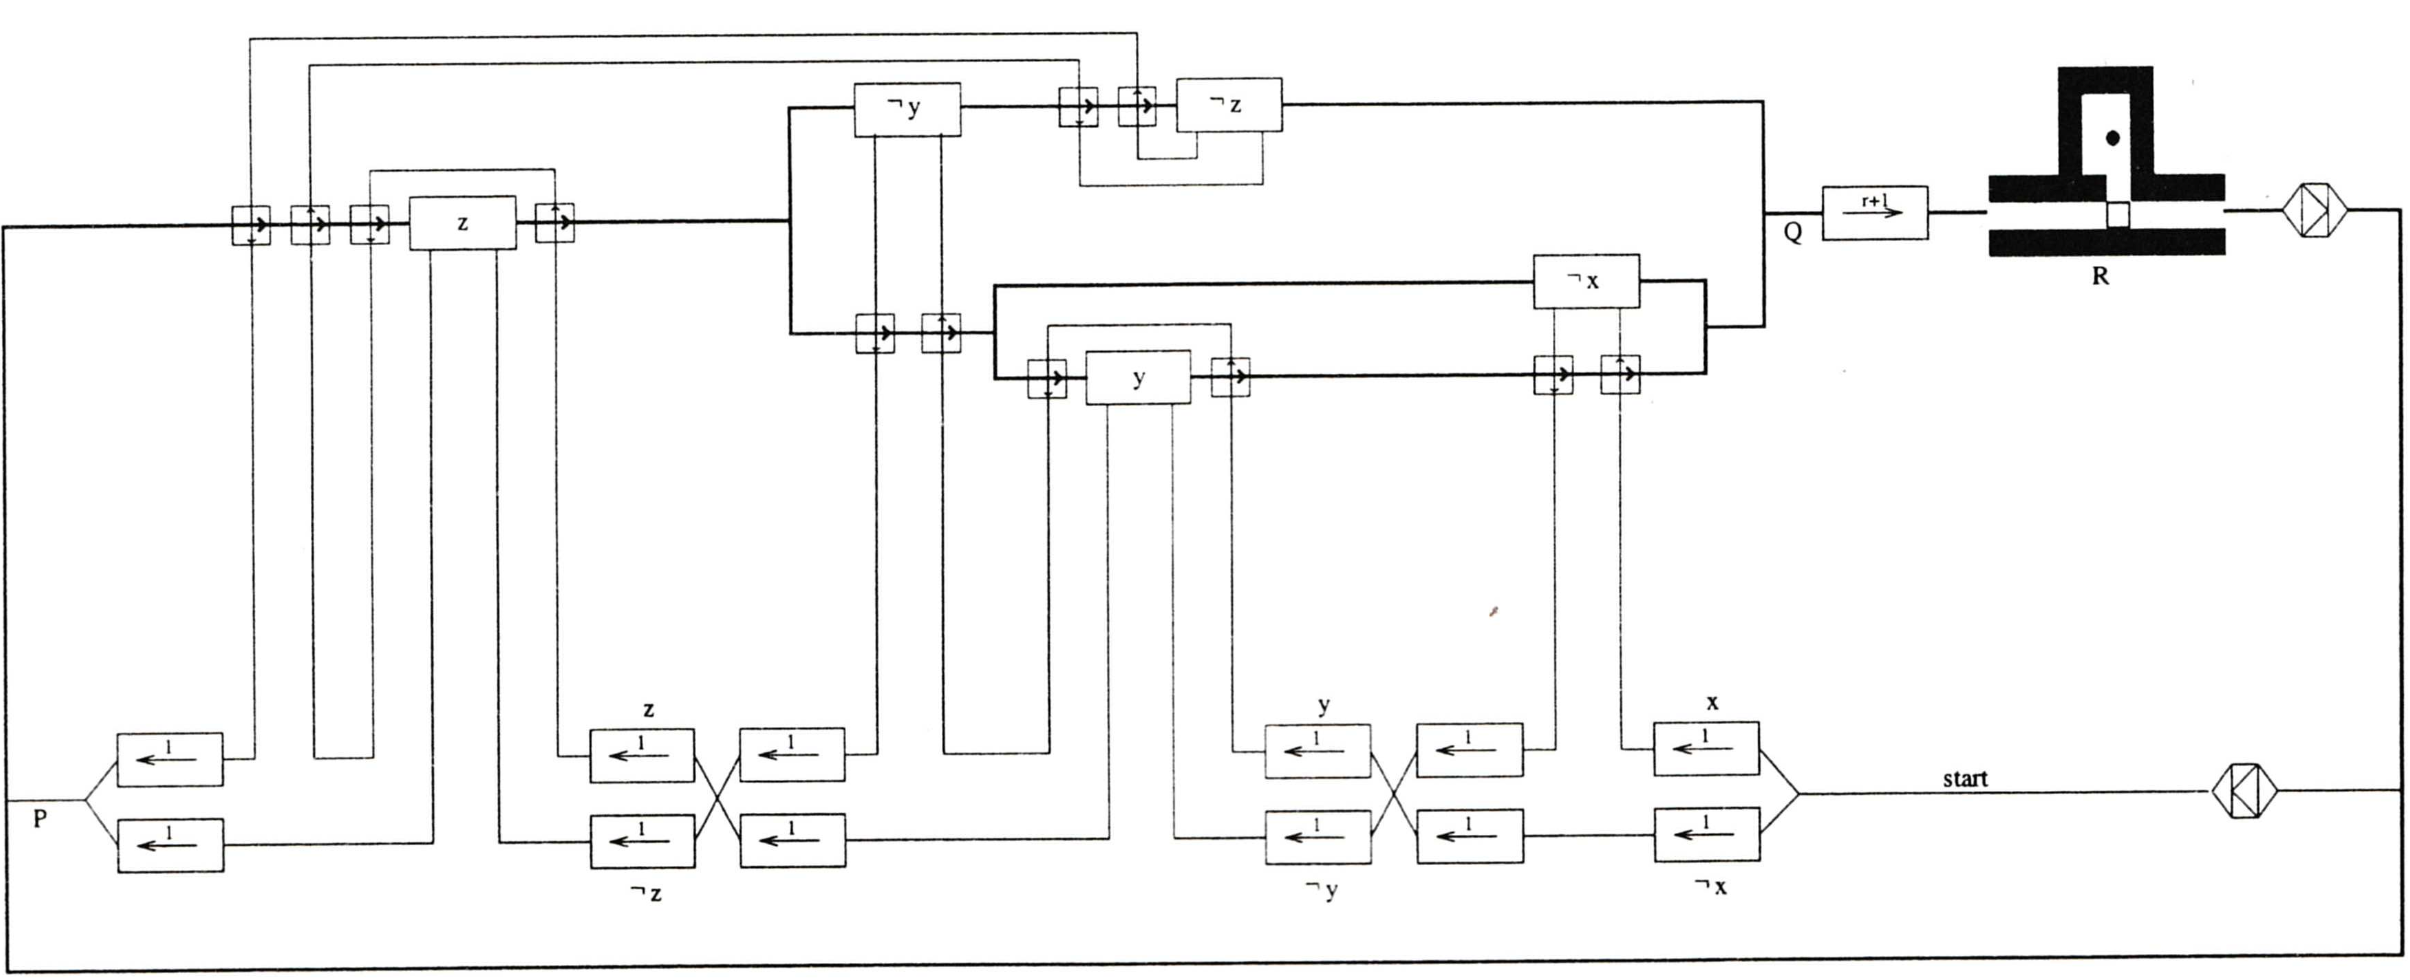
\includegraphics[width=1.2\textwidth, angle=90]{images/nphard-7.png} 
    \caption{}
    \label{fig:b_implementation}
\end{figure}

\begin{figure}[h] % [h] forces the image to be placed "here"
    \centering
    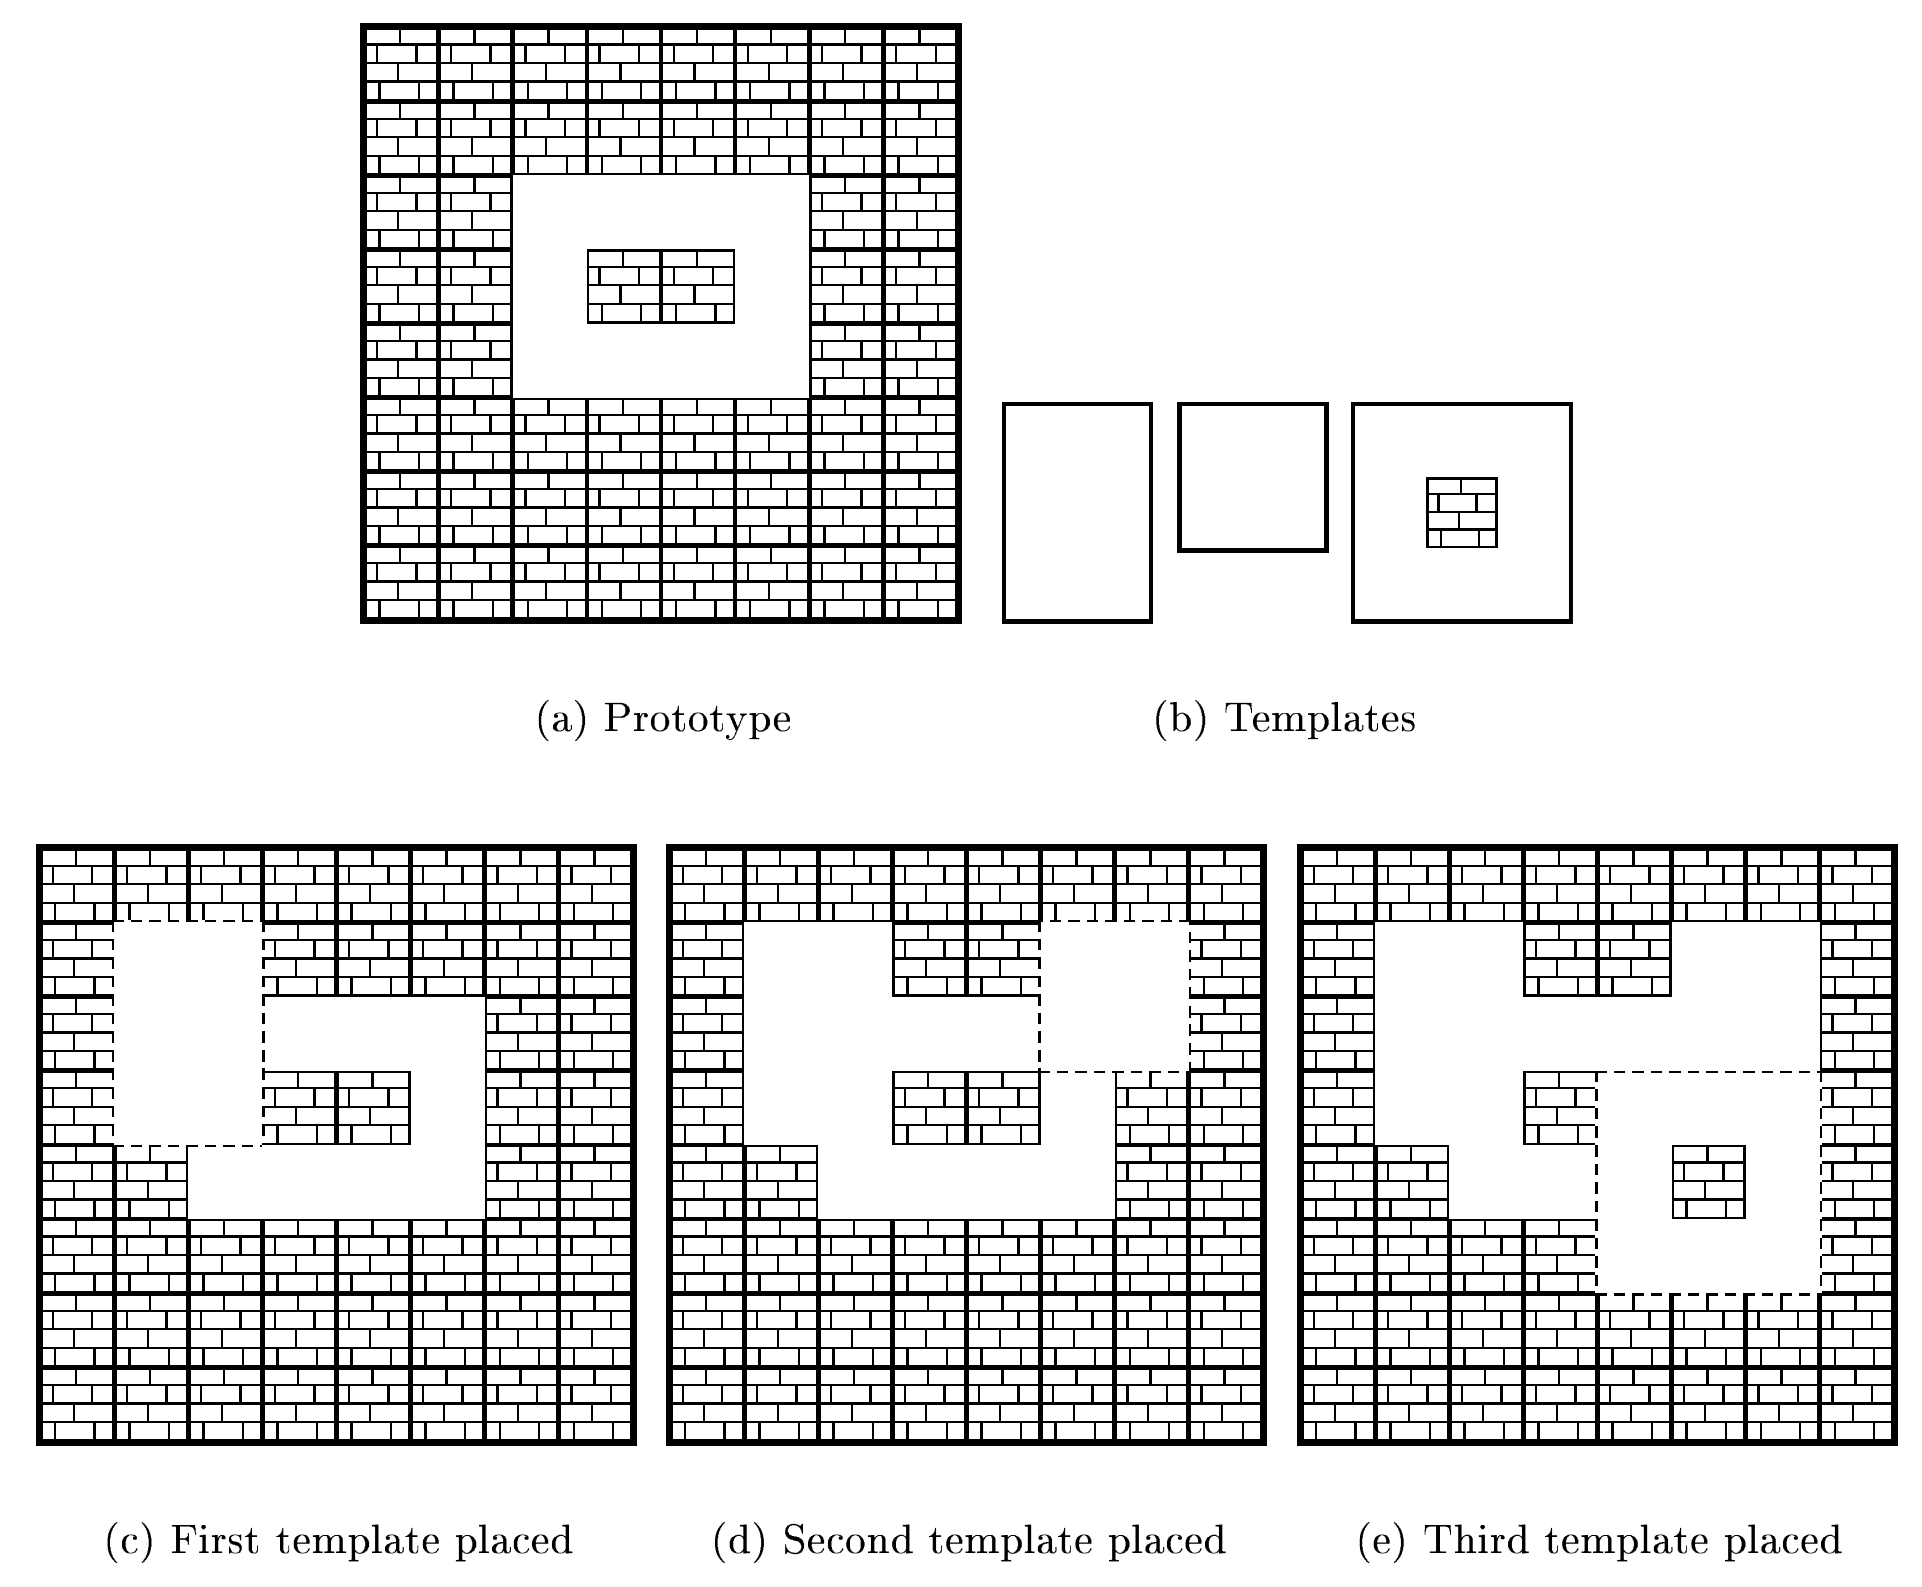
\includegraphics[width=0.9\textwidth]{images/autogeneration1.png}
    \caption{}
    \label{fig:ag1}
\end{figure}

The researchers achieved automatic generation of Sokoban levels through a three-step methodology. First, candidate problems are generated randomly from a prototype and three templates. Next, unsolvable candidates are removed by a Sokoban solver. Finally, trivial or uninteresting candidates are removed by the evaluator. Templates are $2\times 3$, $2\times 2$, and $3\times 3$ empty spaces, used to encourage the generation of multiple paths inside the space. After tiles are placed (Figure \ref{fig:ag1}), there are some tiles where a box can never be placed. These tiles are marked as GOAL\_AVOID (Figure \ref{fig:autogeneration2}). Goal-candidate tiles that are in corners are marked as COR\_GOAL, and the next goal is placed on goal-candidate tiles that are not dead ends and not COR\_GOAL. The dead-end ADD\_AVOID areas are recalculated after every placement.

After the generation of the level, a Breadth-First Search is used to solve the puzzle. While the BFS solver is not able to find solutions to puzzles with long sequences, it can still effectively search for solutions with short sequences \cite{fryers1995sokoban}. Puzzles that cannot be solved are pruned in this step.

The most crucial contribution of this paper is the metric used to determine whether a generated puzzle is non-trivial and interesting. The evaluation program aims to evaluate artistic value using the following criteria:

\begin{center}
    \begin{minipage}{0.8\textwidth} % Adjust width as needed
        \begin{itemize}
            \item Length of solution sequence: if a problem has a very short solution sequence, it is trivial and is rejected. When the length of a problem's solution sequence is less than seven, the problem is rejected.
            \item Number of changes in pushing direction during the solution sequence: in interesting problems, the keeper has to change the direction of pushing objects very often. If the number of changes is less than four, the problem is trivial and must be removed.
            \item Number of detours in the solution sequence: if a problem's solution sequence has no detours, it is uninteresting and is rejected.
        \end{itemize}
    \end{minipage}
\end{center}

The authors claim that these criteria guide the generation of interesting puzzles.


\begin{table}[ht]
    \centering 
    \begin{tabular}{|l|l|l|}
    \hline
    \multicolumn{2}{|l|}{\# of generation failures} & 7 \\ \hline
    \multicolumn{2}{|l|}{\# of problems that have no solutions} & 245 \\ \hline
    \multirow{2}{*}{solvable problems} & removed & 204 \\ \cline{2-3} 
    & outputted & 44 \\ \hline \hline
    \multicolumn{2}{|l|}{\# of trials} & 500 \\ \hline \hline
    \multicolumn{2}{|l|}{real good problems} & 14 \\ \hline
    \end{tabular}
    \caption{Experimental results of the automatic Sokoban generator \cite{murase1996automatic}.}
    \label{table:2}
\end{table}

\begin{figure}[h] % [h] forces the image to be placed "here"
    \centering
    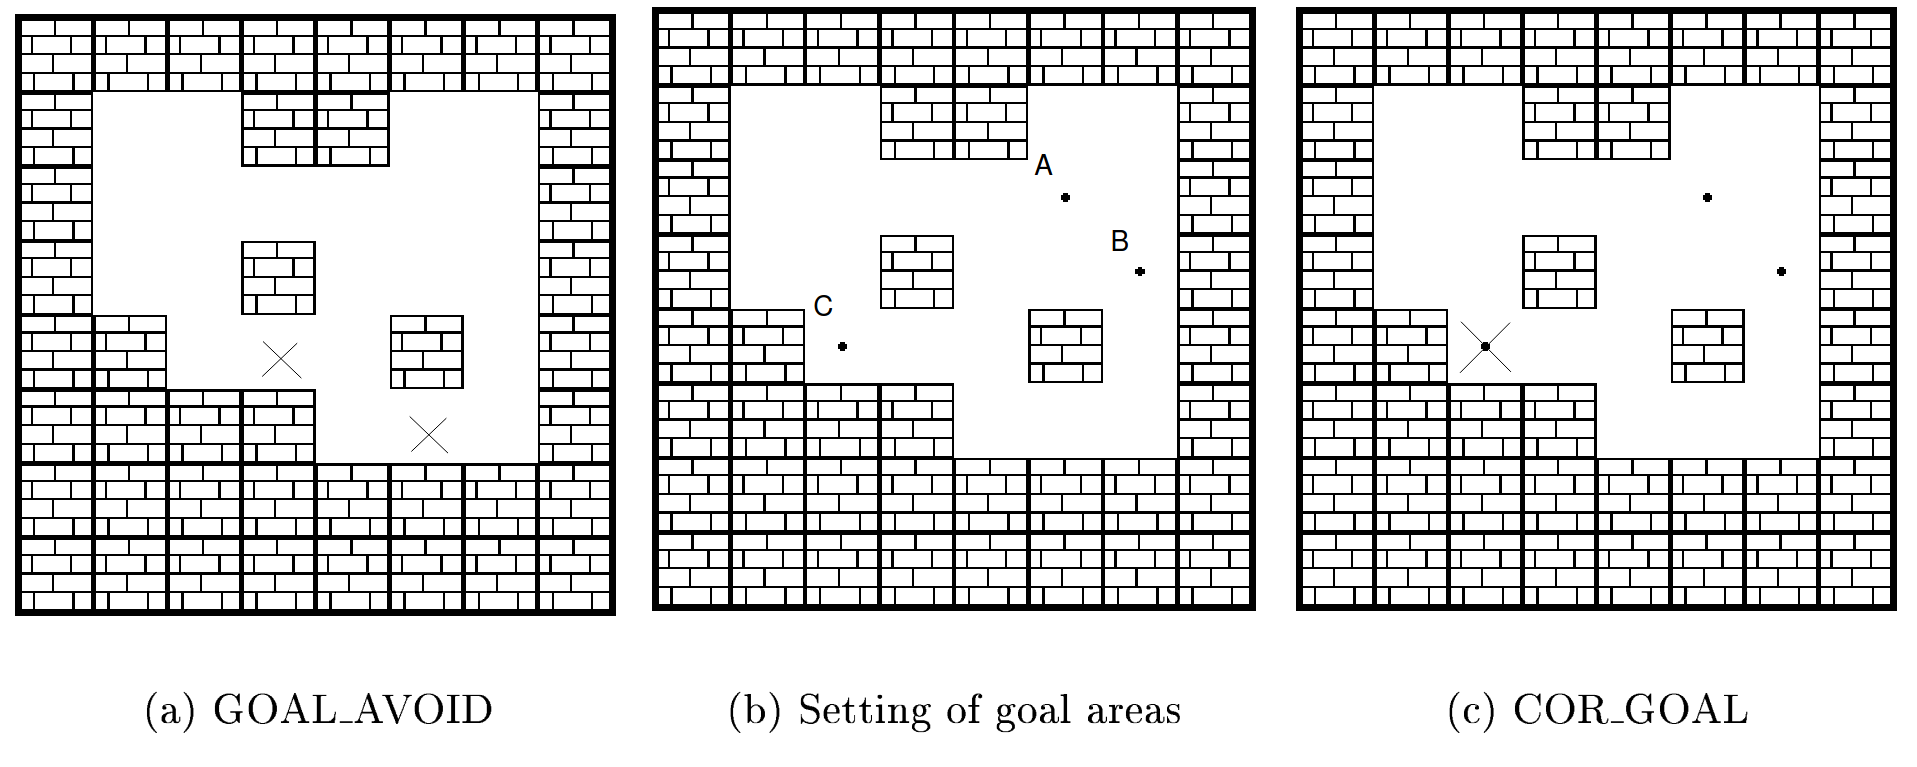
\includegraphics[width=0.9\textwidth]{images/autogeneration2.png} 
    \caption{}
    \label{fig:autogeneration2}
\end{figure}